\documentclass[10pt]{article}

\usepackage[T1]{fontenc}
\usepackage[margin=0.65in]{geometry}
\usepackage{amsmath}
\usepackage{amssymb}
\usepackage{booktabs}
\usepackage{caption}
\usepackage{graphicx}
\usepackage[hidelinks]{hyperref}
\usepackage{longtable}
\usepackage{microtype}

\graphicspath{{figures/}}
\captionsetup{
  font=small,
  labelfont=bf,
  hypcap=false,
  justification=raggedright,
  singlelinecheck=false,
  skip=3pt
}
\setlength{\parindent}{0pt}
\setlength{\parskip}{0.2em}
\setlength{\LTcapwidth}{0.96\textwidth}
\renewcommand{\arraystretch}{1.08}

\begin{document}

\begin{center}
  {\Large\bfseries Rebuttal Figures and Tables}
\end{center}
\vspace{0.5em}

\setcounter{figure}{1}
\begin{center}
  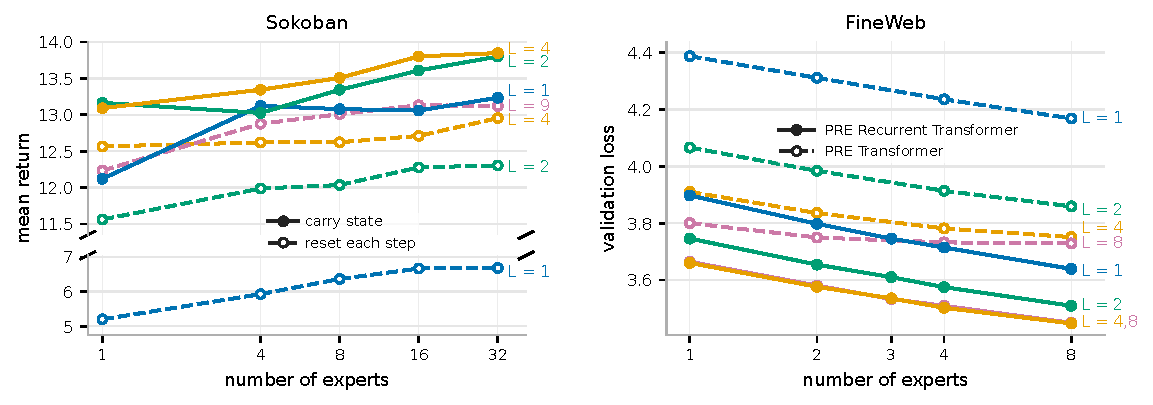
\includegraphics[width=0.93\textwidth]{recurrent_state_sokoban_fineweb.pdf}
\end{center}
\captionof{figure}{
\textbf{Carried state supplies a serial computation axis.}
\textbf{Left}: In Sokoban, solid lines carry hidden state across environment steps and dashed lines reset it every step. Resetting state severely hurts shallow updates, while extra within-step depth partially recovers performance; color denotes within-step depth \(L\).
\textbf{Right}: In FineWeb next-token prediction, the PRE Recurrent Transformer carries latent recurrent state across token steps, while the PRE Transformer recreates latent state from the current segment at each step. The context window size is \(128\) for both architectures.
}
\vspace{0.7em}

\setcounter{figure}{3}
\begin{center}
  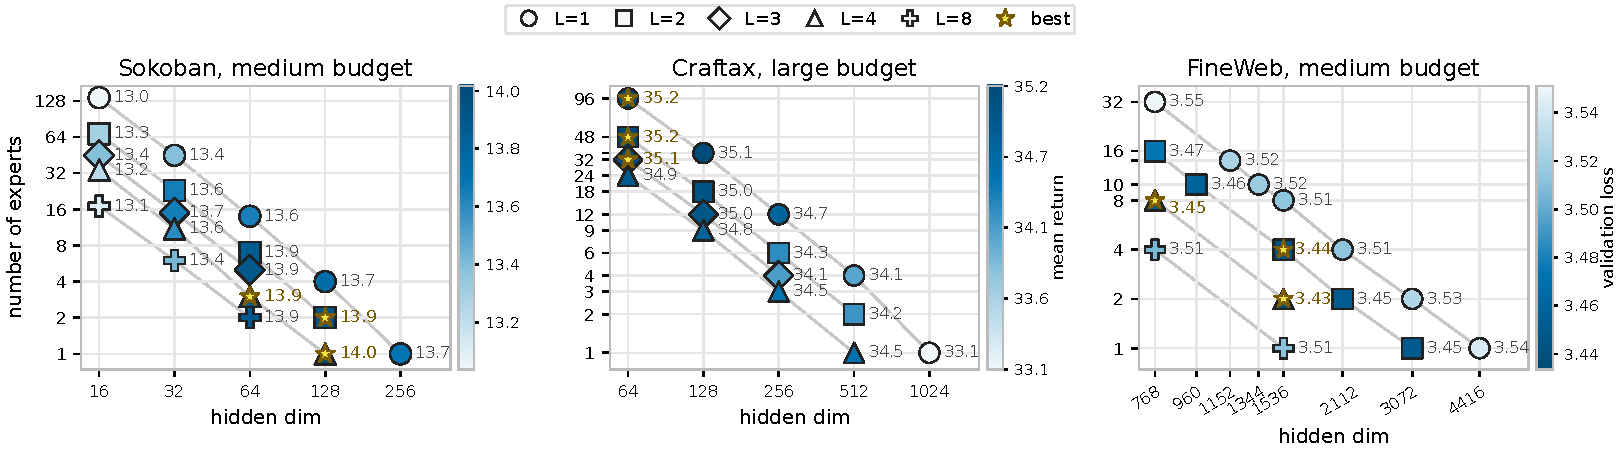
\includegraphics[width=0.93\textwidth]{fixed_compute_allocation_combined_toplegend.pdf}
\end{center}
\captionof{figure}{
\textbf{Fixed-compute allocation across domains.}
The horizontal axis varies expert hidden dimension, the vertical axis varies experts per depth level, and marker shape denotes within-step depth.
}
\clearpage

\setcounter{figure}{4}
\begin{center}
  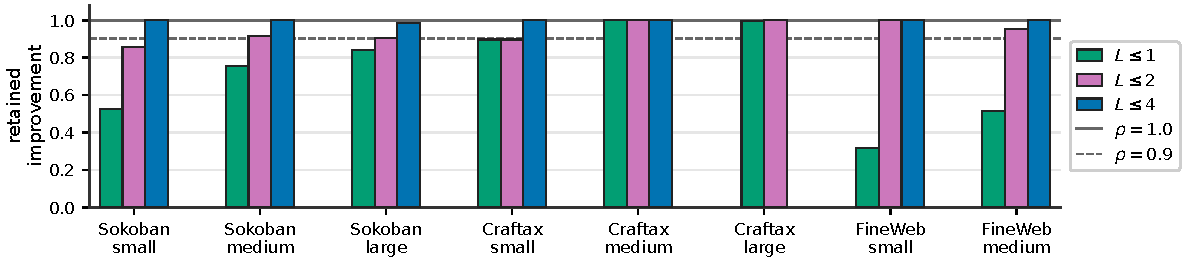
\includegraphics[width=0.88\textwidth]{fixed_compute_retained_improvement.pdf}
\end{center}
\captionof{figure}{
\textbf{Retained improvement under different depth caps.}
Each bar reports the retained-improvement ratio \(\rho_{\leq k}\) for one matched-budget sweep under depth caps \(k \in \{1,2,4,8\}\), with \(Q\) defined as episodic return for Sokoban and Craftax and negative validation cross-entropy for FineWeb.
Horizontal reference lines mark \(\rho=1.00\), which matches the unrestricted best configuration, and \(\rho=0.90\), which retains \(90\%\) of the best improvement over the domain reference.
}
\vspace{0.7em}

\setcounter{table}{0}
\captionof{table}{
\textbf{Best observed performance under within-step depth restrictions in the fixed-compute sweeps.}
Sokoban and Craftax report episodic return, where higher is better. FineWeb next-token prediction reports validation loss, where lower is better. Gap reports the performance loss from the unrestricted optimum: return drop for Sokoban and Craftax, and validation-loss increase for FineWeb. Max \(L\) is the largest within-step depth included in that sweep.
}
\begin{center}
\small
\setlength{\tabcolsep}{4.5pt}
\begin{tabular}{llcccccc}
  \toprule
  Domain & Budget & Max \(L\) & Best overall & Best with \(L \leq 2\) & Gap & Best with \(L \leq 1\) & Gap \\
  \midrule
  Sokoban & small & 8 & 13.665 & 13.552 & 0.113 & 13.287 & 0.378 \\
  Sokoban & medium & 8 & 14.017 & 13.918 & 0.099 & 13.738 & 0.279 \\
  Sokoban & large & 8 & 14.228 & 14.099 & 0.129 & 14.013 & 0.215 \\
  Craftax & small & 8 & 32.436 & 32.436 & 0.000 & 32.436 & 0.000 \\
  Craftax & medium & 8 & 33.934 & 33.934 & 0.000 & 33.802 & 0.132 \\
  Craftax & large & 4 & 35.200 & 35.200 & 0.000 & 35.179 & 0.021 \\
  FineWeb & small & 8 & 3.481 & 3.481 & 0.000 & 3.559 & 0.078 \\
  FineWeb & medium & 8 & 3.434 & 3.441 & 0.007 & 3.511 & 0.078 \\
  \bottomrule
\end{tabular}
\end{center}
\clearpage

\setcounter{figure}{8}
\begin{center}
  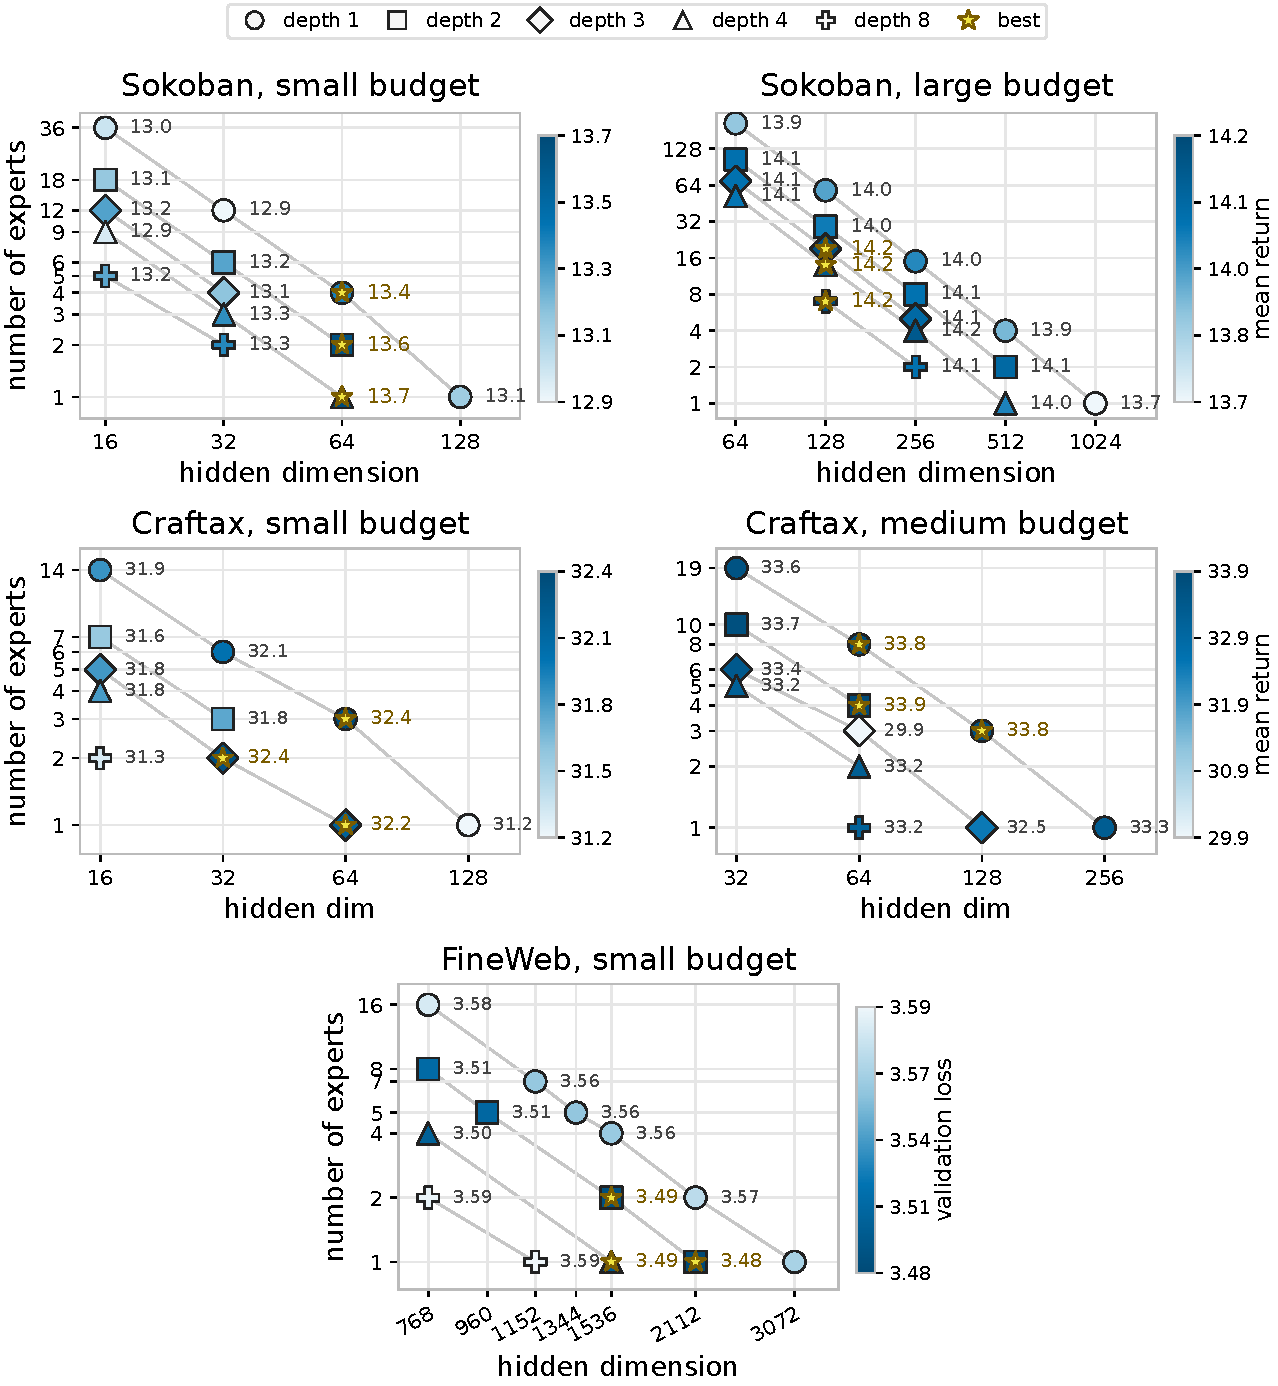
\includegraphics[width=0.62\textwidth]{appendix_fixed_compute_budgets_equal_panels.pdf}
\end{center}
\captionof{figure}{
Additional fixed-compute allocation budgets.
\textbf{Top left}: Sokoban small budget.
\textbf{Top right}: Sokoban large budget.
\textbf{Middle left}: Craftax small budget.
\textbf{Middle right}: Craftax medium budget.
\textbf{Bottom}: FineWeb small budget.
In Sokoban and Craftax, panels vary expert hidden dimension, experts per within-step depth level, and within-step depth; color shows mean return, and only completed or near-completed configurations are shown. In FineWeb, color shows validation loss at the common comparison point of 1.30B consumed tokens, where lower is better.
}
\vspace{0.5em}

\setcounter{table}{1}
\captionof{table}{
\textbf{Fixed-compute budgets.}
Relative work is normalized to the smallest budget within each domain. For Sokoban, \(C(d) \propto d(d+16)\); for Craftax, \(C(d) \propto d(256+2d)\). Best reports the best observed performance in the matched-budget sweep: return for Sokoban and Craftax, and validation loss for FineWeb.
}
\begin{center}
\small
\setlength{\tabcolsep}{3.8pt}
\begin{tabular}{@{}lllcc@{}}
  \toprule
  Domain & Budget & Reference config & Work / small budget & Best \\
  \midrule
  Sokoban & small & \(L=1\), \(E=1\), \(d=128\) & \(1.00\) & \(13.665\) \\
  Sokoban & medium & \(L=1\), \(E=1\), \(d=256\) & \(3.78\) & \(14.017\) \\
  Sokoban & large & \(L=1\), \(E=1\), \(d=1024\) & \(57.78\) & \(14.228\) \\
  Craftax & small & \(L=1\), \(E=1\), \(d=128\) & \(1.00\) & \(32.436\) \\
  Craftax & medium & \(L=1\), \(E=1\), \(d=256\) & \(3.00\) & \(33.934\) \\
  Craftax & large & \(L=1\), \(E=1\), \(d=1024\) & \(36.00\) & \(35.200\) \\
  FineWeb & small & \(L=16, E=1\), \(d=768\) & \(1.00\) & \(3.481\) \\
  FineWeb & medium & \(L=32, E=1\), \(d=768\) & \(2.00\) & \(3.434\) \\
  \bottomrule
\end{tabular}
\end{center}
\clearpage

\setcounter{table}{2}
\captionof{table}{
\textbf{Best exact-depth comparison, \(L=4\) versus \(L=2\).}
For each depth, the configuration with the best observed mean higher-is-better score \(Q\) is selected. \(\Delta Q\) is the observed difference between sample means \(\bar Q_4-\bar Q_2\), so positive values favor \(L=4\). The \(p\)-value is from Welch's \(t\)-test of \(H_0:\mathbb{E}[Q_4]\leq\mathbb{E}[Q_2]\) against \(H_1:\mathbb{E}[Q_4]>\mathbb{E}[Q_2]\). \(n_4/n_2\) gives the numbers of independent runs for the two configurations.
}
\begin{center}
\small
\setlength{\tabcolsep}{4.0pt}
\begin{tabular}{@{}llllrrr@{}}
  \toprule
  Domain & Budget & Best \(L=4\) & Best \(L=2\) & \(\Delta Q\) & \(n_4/n_2\) & \(p\) \\
  \midrule
  Sokoban & small & \(E=1,d=64\) & \(E=2,d=64\) & 0.113 & 9/9 & 0.0150 \\
  Sokoban & medium & \(E=1,d=128\) & \(E=2,d=128\) & 0.099 & 9/9 & 0.0060 \\
  Sokoban & large & \(E=14,d=128\) & \(E=2,d=512\) & 0.074 & 3/3 & 0.1005 \\
  Craftax & small & \(E=4,d=16\) & \(E=3,d=32\) & 0.063 & 3/3 & 0.4407 \\
  Craftax & medium & \(E=2,d=64\) & \(E=4,d=64\) & -0.690 & 3/3 & 0.9275 \\
  Craftax & large & \(E=24,d=64\) & \(E=48,d=64\) & -0.266 & 3/3 & 0.8364 \\
  \bottomrule
\end{tabular}
\end{center}
\vspace{0.5em}

\setcounter{table}{3}
\captionof{table}{
\textbf{Best exact-depth comparison, \(L=2\) versus \(L=1\).}
For each depth, the configuration with the best observed mean higher-is-better score \(Q\) is selected. \(\Delta Q\) is the observed difference between sample means \(\bar Q_2-\bar Q_1\), so positive values favor \(L=2\). The \(p\)-value is from Welch's \(t\)-test of \(H_0:\mathbb{E}[Q_2]\leq\mathbb{E}[Q_1]\) against \(H_1:\mathbb{E}[Q_2]>\mathbb{E}[Q_1]\). \(n_2/n_1\) gives the numbers of independent runs for the two configurations.
}
\begin{center}
\small
\setlength{\tabcolsep}{4.0pt}
\begin{tabular}{@{}llllrrr@{}}
  \toprule
  Domain & Budget & Best \(L=2\) & Best \(L=1\) & \(\Delta Q\) & \(n_2/n_1\) & \(p\) \\
  \midrule
  Sokoban & small & \(E=2,d=64\) & \(E=4,d=64\) & 0.265 & 9/9 & \(<0.0001\) \\
  Sokoban & medium & \(E=2,d=128\) & \(E=4,d=128\) & 0.180 & 9/9 & \(<0.0001\) \\
  Sokoban & large & \(E=2,d=512\) & \(E=15,d=256\) & 0.086 & 3/3 & 0.0745 \\
  Craftax & small & \(E=3,d=32\) & \(E=3,d=64\) & -0.670 & 3/3 & 0.8968 \\
  Craftax & medium & \(E=4,d=64\) & \(E=8,d=64\) & 0.132 & 3/3 & 0.3551 \\
  Craftax & large & \(E=48,d=64\) & \(E=96,d=64\) & 0.021 & 3/3 & 0.4545 \\
  \bottomrule
\end{tabular}
\end{center}
\vspace{0.5em}

\setcounter{table}{4}
\captionof{table}{
\textbf{Best \(L=4\) versus all \(L=2\) configurations in Sokoban.}
For each small and medium budget, the \(L=4\) configuration with the best observed mean return is compared with every \(L=2\) configuration. Positive \(\Delta Q\) favors \(L=4\), and \(p\) is from the one-sided Welch test defined above. \(n_4/n_2\) gives the numbers of independent runs for the \(L=4\) and \(L=2\) configurations.
}
\begin{center}
\small
\setlength{\tabcolsep}{5.0pt}
\begin{tabular}{@{}lllrrr@{}}
  \toprule
  Budget & Best \(L=4\) & \(L=2\) configuration & \(\Delta Q\) & \(n_4/n_2\) & \(p\) \\
  \midrule
  small & \(E=1,d=64\) & \(E=2,d=64\) & 0.113 & 9/9 & 0.0150 \\
  small & \(E=1,d=64\) & \(E=6,d=32\) & 0.468 & 9/9 & \(<0.0001\) \\
  small & \(E=1,d=64\) & \(E=18,d=16\) & 0.658 & 9/9 & \(<0.0001\) \\
  medium & \(E=1,d=128\) & \(E=2,d=128\) & 0.099 & 9/9 & 0.0060 \\
  medium & \(E=1,d=128\) & \(E=7,d=64\) & 0.151 & 9/9 & \(<0.0001\) \\
  medium & \(E=1,d=128\) & \(E=23,d=32\) & 0.375 & 9/9 & \(<0.0001\) \\
  medium & \(E=1,d=128\) & \(E=68,d=16\) & 0.730 & 9/9 & \(<0.0001\) \\
  \bottomrule
\end{tabular}
\end{center}
\vspace{0.5em}

\setcounter{table}{5}
\captionof{table}{
\textbf{Best \(L=2\) versus all \(L=1\) configurations in Sokoban.}
For each small and medium budget, the \(L=2\) configuration with the best observed mean return is compared with every \(L=1\) configuration. Positive \(\Delta Q\) favors \(L=2\), and \(p\) is from the one-sided Welch test defined above. \(n_2/n_1\) gives the numbers of independent runs for the \(L=2\) and \(L=1\) configurations.
}
\begin{center}
\small
\setlength{\tabcolsep}{5.0pt}
\begin{tabular}{@{}lllrrr@{}}
  \toprule
  Budget & Best \(L=2\) & \(L=1\) configuration & \(\Delta Q\) & \(n_2/n_1\) & \(p\) \\
  \midrule
  small & \(E=2,d=64\) & \(E=4,d=64\) & 0.265 & 9/9 & \(<0.0001\) \\
  small & \(E=2,d=64\) & \(E=1,d=128\) & 0.481 & 9/7 & 0.0002 \\
  small & \(E=2,d=64\) & \(E=12,d=32\) & 0.624 & 9/9 & \(<0.0001\) \\
  small & \(E=2,d=64\) & \(E=36,d=16\) & 0.688 & 9/9 & \(<0.0001\) \\
  medium & \(E=2,d=128\) & \(E=4,d=128\) & 0.180 & 9/9 & \(<0.0001\) \\
  medium & \(E=2,d=128\) & \(E=1,d=256\) & 0.231 & 9/9 & \(<0.0001\) \\
  medium & \(E=2,d=128\) & \(E=14,d=64\) & 0.277 & 9/9 & \(<0.0001\) \\
  medium & \(E=2,d=128\) & \(E=45,d=32\) & 0.534 & 9/9 & \(<0.0001\) \\
  medium & \(E=2,d=128\) & \(E=136,d=16\) & 0.881 & 9/9 & \(<0.0001\) \\
  \bottomrule
\end{tabular}
\end{center}
\clearpage

The Sokoban small- and medium-budget rows contain nine runs, except for the
small-budget \(L=1,E=1,d=128\) anchor, which contains seven. Seeds 7 and 9 for
that anchor ended below the established \(94.2\%\) training-progress cutoff
and are excluded. Large-budget Sokoban and Craftax use the available three
runs.

\setcounter{table}{6}
% Generated by scripts/build_fixed_compute_seed_tables.py.

{\scriptsize
\setlength{\tabcolsep}{1.2pt}
\begin{longtable}{@{}lrrrrrrrrrrrrrr@{}}
\caption{\textbf{Per-seed Sokoban small- and medium-budget fixed-compute results.} These are all points shown for this benchmark in Figures 4 and 9. Each seed entry is the mean of the final five logged episodic returns. Mean and standard error are computed across the available seed values. Columns \(s_1,\ldots,s_9\) identify random seeds.}\label{tab:appendix-sokoban-fixed-compute-seeds}\\
\toprule
Budget & \(L\) & \(E\) & \(d\) & \(s_1\) & \(s_2\) & \(s_3\) & \(s_4\) & \(s_5\) & \(s_6\) & \(s_7\) & \(s_8\) & \(s_9\) & Mean & SE \\
\midrule
\endfirsthead
\multicolumn{15}{c}{\tablename~\thetable\ (continued)} \\
\toprule
Budget & \(L\) & \(E\) & \(d\) & \(s_1\) & \(s_2\) & \(s_3\) & \(s_4\) & \(s_5\) & \(s_6\) & \(s_7\) & \(s_8\) & \(s_9\) & Mean & SE \\
\midrule
\endhead
\midrule
\multicolumn{15}{r}{Continued on next page} \\
\endfoot
\bottomrule
\endlastfoot
small & 1 & 1 & 128 & 12.874 & 13.109 & 13.269 & 12.726 & 13.146 & 13.063 & 13.366 & 13.313 & 13.003 & 13.096 & 0.070 \\
small & 1 & 4 & 64 & 13.381 & 13.174 & 13.499 & 13.164 & 13.195 & 13.196 & 13.309 & 13.332 & 13.334 & 13.287 & 0.038 \\
small & 1 & 12 & 32 & 12.755 & 12.926 & 12.909 & 13.052 & 13.096 & 12.947 & 13.003 & 12.787 & 12.875 & 12.928 & 0.038 \\
small & 1 & 36 & 16 & 12.796 & 13.082 & 13.020 & 13.203 & 12.969 & 12.945 & 12.702 & 12.517 & 12.549 & 12.865 & 0.079 \\
small & 2 & 2 & 64 & 13.620 & 13.700 & 13.518 & 13.643 & 13.345 & 13.553 & 13.536 & 13.423 & 13.631 & 13.552 & 0.038 \\
small & 2 & 6 & 32 & 13.223 & 13.185 & 13.296 & 13.080 & 13.178 & 13.017 & 13.121 & 13.380 & 13.297 & 13.198 & 0.038 \\
small & 2 & 18 & 16 & 13.172 & 13.124 & 13.022 & 13.214 & 12.515 & 12.964 & 12.836 & 13.289 & 12.931 & 13.008 & 0.078 \\
small & 3 & 4 & 32 & 12.963 & 13.223 & 13.195 & 13.007 & 12.995 & 13.141 & 13.146 & 13.005 & 13.407 & 13.120 & 0.048 \\
small & 3 & 12 & 16 & 13.155 & 13.485 & 13.082 & 13.177 & 13.175 & 13.161 & 12.883 & 13.023 & 12.981 & 13.125 & 0.056 \\
small & 4 & 1 & 64 & 13.559 & 13.757 & 13.660 & 13.775 & 13.689 & 13.605 & 13.687 & 13.530 & 13.727 & 13.665 & 0.029 \\
small & 4 & 3 & 32 & 13.415 & 13.370 & 13.130 & 13.087 & 13.092 & 13.013 & 13.098 & 13.257 & 13.301 & 13.196 & 0.048 \\
small & 4 & 9 & 16 & 12.703 & 13.142 & 12.948 & 12.890 & 12.860 & 13.133 & 12.966 & 13.098 & 13.161 & 12.989 & 0.052 \\
small & 8 & 2 & 32 & 13.273 & 13.252 & 13.324 & 13.221 & 13.124 & 13.238 & 13.150 & 12.905 & 13.211 & 13.189 & 0.041 \\
small & 8 & 5 & 16 & 13.516 & 13.325 & 12.831 & 13.521 & 13.296 & 13.071 & 13.108 & 13.183 & 13.514 & 13.263 & 0.079 \\
medium & 1 & 1 & 256 & 13.713 & 13.635 & 13.750 & 13.737 & 13.803 & 13.593 & 13.703 & 13.596 & 13.654 & 13.687 & 0.024 \\
medium & 1 & 4 & 128 & 13.672 & 13.722 & 13.860 & 13.715 & 13.805 & 13.753 & 13.756 & 13.742 & 13.613 & 13.738 & 0.024 \\
medium & 1 & 14 & 64 & 13.674 & 13.652 & 13.646 & 13.730 & 13.596 & 13.667 & 13.631 & 13.478 & 13.696 & 13.641 & 0.024 \\
medium & 1 & 45 & 32 & 13.422 & 13.281 & 13.384 & 13.482 & 13.186 & 13.315 & 13.443 & 13.372 & 13.564 & 13.383 & 0.038 \\
medium & 1 & 136 & 16 & 13.097 & 13.130 & 13.101 & 12.942 & 13.072 & 13.035 & 12.949 & 12.849 & 13.158 & 13.037 & 0.034 \\
medium & 2 & 2 & 128 & 13.862 & 13.868 & 13.986 & 13.845 & 13.823 & 13.962 & 13.881 & 14.068 & 13.965 & 13.918 & 0.027 \\
medium & 2 & 7 & 64 & 13.873 & 13.821 & 13.890 & 13.917 & 13.893 & 13.777 & 13.795 & 13.896 & 13.935 & 13.866 & 0.019 \\
medium & 2 & 23 & 32 & 13.656 & 13.576 & 13.784 & 13.670 & 13.594 & 13.541 & 13.713 & 13.668 & 13.577 & 13.642 & 0.026 \\
medium & 2 & 68 & 16 & 13.349 & 13.436 & 13.109 & 13.278 & 13.443 & 13.475 & 13.214 & 13.085 & 13.198 & 13.287 & 0.049 \\
medium & 3 & 5 & 64 & 13.905 & 13.899 & 13.838 & 14.056 & 13.783 & 13.885 & 13.884 & 13.913 & 13.932 & 13.899 & 0.025 \\
medium & 3 & 15 & 32 & 13.781 & 13.524 & 13.604 & 13.781 & 13.684 & 13.385 & 13.475 & 13.833 & 13.806 & 13.653 & 0.054 \\
medium & 3 & 45 & 16 & 13.150 & 13.451 & 13.194 & 13.537 & 13.449 & 13.466 & 13.450 & 13.417 & 13.350 & 13.385 & 0.044 \\
medium & 4 & 1 & 128 & 13.970 & 14.079 & 13.974 & 14.074 & 13.958 & 14.025 & 13.914 & 14.109 & 14.050 & 14.017 & 0.022 \\
medium & 4 & 3 & 64 & 13.833 & 14.091 & 13.875 & 13.761 & 13.736 & 14.068 & 13.967 & 14.129 & 13.802 & 13.918 & 0.050 \\
medium & 4 & 11 & 32 & 13.624 & 13.596 & 13.726 & 13.587 & 13.428 & 13.578 & 13.631 & 13.632 & 13.504 & 13.590 & 0.028 \\
medium & 4 & 34 & 16 & 13.039 & 13.434 & 13.324 & 13.162 & 13.107 & 13.230 & 13.178 & 13.295 & 13.211 & 13.220 & 0.040 \\
medium & 8 & 2 & 64 & 14.012 & 13.900 & 13.884 & 13.718 & 13.864 & 13.869 & 14.036 & 13.658 & 14.102 & 13.894 & 0.048 \\
medium & 8 & 6 & 32 & 13.644 & 13.339 & 13.385 & 13.601 & 12.965 & 13.221 & 13.366 & 13.581 & 13.626 & 13.414 & 0.075 \\
medium & 8 & 17 & 16 & 13.074 & 13.384 & 13.148 & 13.400 & 12.863 & 13.178 & 12.924 & 12.843 & 13.128 & 13.105 & 0.068 \\
\end{longtable}
}

{\scriptsize
\setlength{\tabcolsep}{3.0pt}
\begin{longtable}{@{}lrrrrrrrr@{}}
\caption{\textbf{Per-seed Sokoban large-budget fixed-compute results.} These are all points shown for this benchmark in Figures 4 and 9. Each seed entry is the mean of the final five logged episodic returns. Mean and standard error are computed across the available seed values. Columns \(s_1,\ldots,s_3\) identify random seeds.}\label{tab:appendix-sokoban-large-fixed-compute-seeds}\\
\toprule
Budget & \(L\) & \(E\) & \(d\) & \(s_1\) & \(s_2\) & \(s_3\) & Mean & SE \\
\midrule
\endfirsthead
\multicolumn{9}{c}{\tablename~\thetable\ (continued)} \\
\toprule
Budget & \(L\) & \(E\) & \(d\) & \(s_1\) & \(s_2\) & \(s_3\) & Mean & SE \\
\midrule
\endhead
\midrule
\multicolumn{9}{r}{Continued on next page} \\
\endfoot
\bottomrule
\endlastfoot
large & 1 & 1 & 1024 & 13.783 & 13.573 & 13.790 & 13.715 & 0.071 \\
large & 1 & 4 & 512 & 13.907 & 13.862 & 13.971 & 13.914 & 0.032 \\
large & 1 & 15 & 256 & 14.004 & 13.999 & 14.035 & 14.013 & 0.011 \\
large & 1 & 58 & 128 & 13.990 & 13.852 & 14.027 & 13.956 & 0.053 \\
large & 1 & 208 & 64 & 13.809 & 13.931 & 13.891 & 13.877 & 0.036 \\
large & 2 & 2 & 512 & 14.051 & 14.070 & 14.176 & 14.099 & 0.039 \\
large & 2 & 8 & 256 & 14.141 & 13.899 & 14.148 & 14.063 & 0.082 \\
large & 2 & 29 & 128 & 14.048 & 13.974 & 14.102 & 14.041 & 0.037 \\
large & 2 & 104 & 64 & 14.063 & 14.067 & 14.079 & 14.070 & 0.005 \\
large & 3 & 5 & 256 & 14.142 & 14.057 & 14.090 & 14.096 & 0.025 \\
large & 3 & 19 & 128 & 14.232 & 14.168 & 14.226 & 14.209 & 0.020 \\
large & 3 & 69 & 64 & 13.988 & 14.103 & 14.104 & 14.065 & 0.039 \\
large & 4 & 1 & 512 & 13.957 & 14.104 & 14.007 & 14.022 & 0.043 \\
large & 4 & 4 & 256 & 14.194 & 14.089 & 14.208 & 14.164 & 0.037 \\
large & 4 & 14 & 128 & 14.125 & 14.214 & 14.179 & 14.173 & 0.026 \\
large & 4 & 52 & 64 & 14.042 & 14.035 & 14.081 & 14.053 & 0.014 \\
large & 8 & 2 & 256 & 14.143 & 14.039 & 14.010 & 14.064 & 0.040 \\
large & 8 & 7 & 128 & 14.145 & 14.281 & 14.259 & 14.228 & 0.042 \\
\end{longtable}
}

{\scriptsize
\setlength{\tabcolsep}{3.0pt}
\begin{longtable}{@{}lrrrrrrrr@{}}
\caption{\textbf{Per-seed Craftax fixed-compute results.} These are all points shown for this benchmark in Figures 4 and 9. Each seed entry is the mean of the final five logged episodic returns. Mean and standard error are computed across the available seed values. Columns \(s_1,\ldots,s_3\) identify random seeds.}\label{tab:appendix-craftax-fixed-compute-seeds}\\
\toprule
Budget & \(L\) & \(E\) & \(d\) & \(s_1\) & \(s_2\) & \(s_3\) & Mean & SE \\
\midrule
\endfirsthead
\multicolumn{9}{c}{\tablename~\thetable\ (continued)} \\
\toprule
Budget & \(L\) & \(E\) & \(d\) & \(s_1\) & \(s_2\) & \(s_3\) & Mean & SE \\
\midrule
\endhead
\midrule
\multicolumn{9}{r}{Continued on next page} \\
\endfoot
\bottomrule
\endlastfoot
small & 1 & 1 & 128 & 29.480 & 31.632 & 32.538 & 31.216 & 0.907 \\
small & 1 & 3 & 64 & 32.367 & 32.800 & 32.142 & 32.436 & 0.193 \\
small & 1 & 6 & 32 & 31.592 & 32.166 & 32.393 & 32.050 & 0.238 \\
small & 1 & 14 & 16 & 31.771 & 31.964 & 31.866 & 31.867 & 0.056 \\
small & 2 & 3 & 32 & 32.132 & 32.141 & 31.026 & 31.766 & 0.370 \\
small & 2 & 7 & 16 & 31.171 & 31.600 & 31.977 & 31.582 & 0.233 \\
small & 3 & 1 & 64 & 32.755 & 31.168 & 32.701 & 32.208 & 0.520 \\
small & 3 & 2 & 32 & 32.198 & 32.390 & 32.557 & 32.381 & 0.104 \\
small & 3 & 5 & 16 & 32.047 & 31.144 & 32.337 & 31.843 & 0.359 \\
small & 4 & 4 & 16 & 31.927 & 31.769 & 31.791 & 31.829 & 0.049 \\
small & 8 & 2 & 16 & 31.191 & 31.510 & 31.252 & 31.318 & 0.098 \\
medium & 1 & 1 & 256 & 33.611 & 33.255 & 33.034 & 33.300 & 0.168 \\
medium & 1 & 3 & 128 & 33.481 & 33.792 & 34.011 & 33.761 & 0.154 \\
medium & 1 & 8 & 64 & 33.573 & 33.952 & 33.881 & 33.802 & 0.116 \\
medium & 1 & 19 & 32 & 33.299 & 33.933 & 33.635 & 33.622 & 0.183 \\
medium & 2 & 4 & 64 & 34.372 & 34.060 & 33.370 & 33.934 & 0.296 \\
medium & 2 & 10 & 32 & 33.556 & 33.955 & 33.658 & 33.723 & 0.120 \\
medium & 3 & 1 & 128 & 33.713 & 30.396 & 33.326 & 32.478 & 1.047 \\
medium & 3 & 3 & 64 & 34.636 & 21.646 & 33.337 & 29.873 & 4.130 \\
medium & 3 & 6 & 32 & 33.660 & 33.012 & 33.606 & 33.426 & 0.207 \\
medium & 4 & 2 & 64 & 32.895 & 33.153 & 33.685 & 33.244 & 0.233 \\
medium & 4 & 5 & 32 & 33.349 & 32.919 & 33.252 & 33.173 & 0.130 \\
medium & 8 & 1 & 64 & 33.488 & 33.150 & 32.814 & 33.150 & 0.194 \\
large & 1 & 1 & 1024 & 33.044 & 34.154 & 31.969 & 33.056 & 0.631 \\
large & 1 & 4 & 512 & 33.405 & 34.443 & 34.306 & 34.051 & 0.326 \\
large & 1 & 12 & 256 & 34.329 & 34.919 & 34.959 & 34.736 & 0.204 \\
large & 1 & 36 & 128 & 35.190 & 35.049 & 35.172 & 35.137 & 0.044 \\
large & 1 & 96 & 64 & 35.228 & 35.285 & 35.024 & 35.179 & 0.079 \\
large & 2 & 2 & 512 & 34.128 & 34.553 & 33.895 & 34.192 & 0.193 \\
large & 2 & 6 & 256 & 34.223 & 33.614 & 34.942 & 34.260 & 0.384 \\
large & 2 & 18 & 128 & 34.646 & 34.683 & 35.735 & 35.021 & 0.357 \\
large & 2 & 48 & 64 & 35.490 & 35.131 & 34.980 & 35.200 & 0.151 \\
large & 3 & 4 & 256 & 33.728 & 34.438 & 34.156 & 34.107 & 0.206 \\
large & 3 & 12 & 128 & 34.878 & 35.186 & 34.882 & 34.982 & 0.102 \\
large & 3 & 32 & 64 & 34.726 & 35.700 & 34.995 & 35.140 & 0.291 \\
large & 4 & 1 & 512 & 34.670 & 34.525 & 34.392 & 34.529 & 0.080 \\
large & 4 & 3 & 256 & 34.273 & 34.422 & 34.738 & 34.477 & 0.137 \\
large & 4 & 9 & 128 & 34.966 & 34.542 & 34.787 & 34.765 & 0.123 \\
large & 4 & 24 & 64 & 35.020 & 34.583 & 35.199 & 34.934 & 0.183 \\
\end{longtable}
}

\clearpage

\setcounter{figure}{11}
\begin{center}
  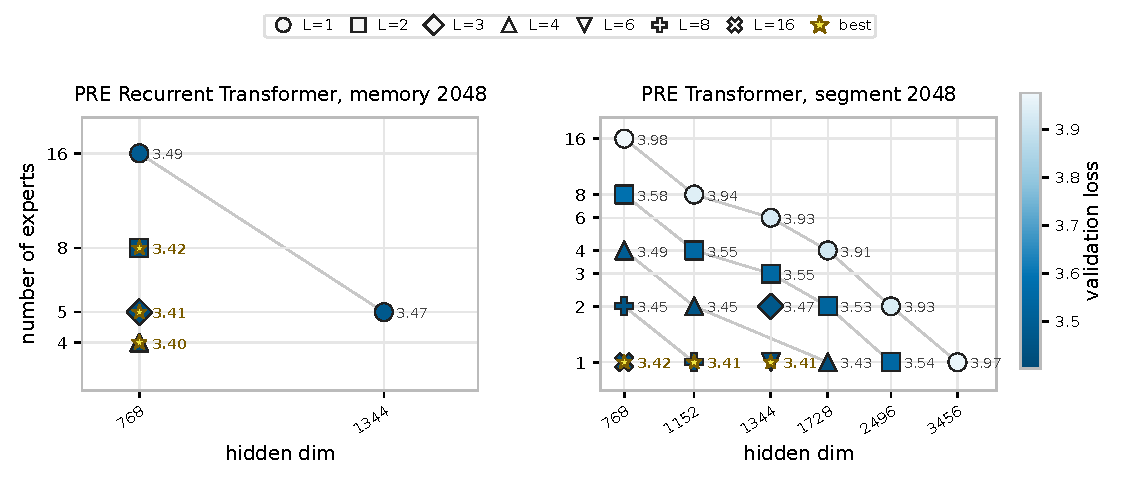
\includegraphics[width=0.88\textwidth]{language_model_recmoe_vs_gptmoe_budget16_2048.pdf}
\end{center}
\captionof{figure}{
FineWeb budget-16 comparison at long context.
\textbf{Left}: completed finite PRE Recurrent Transformer runs with recurrent memory length 2048 and segment length of 64.
\textbf{Right}: the corresponding non-recurrent GPT-style PRE Transformer fixed-budget sweep with training segment length 2048.
Color and point labels show validation loss at the latest common logged validation point within each panel, where lower is better; marker shape denotes within-step depth \(L\), and stars mark the best configurations within each panel. The PRE Recurrent Transformer panel contains the subset of memory-2048 configurations that completed with finite validation loss, while the GPT-style PRE Transformer panel contains the completed segment-2048 sweep.
}
\vspace{0.7em}

\setcounter{figure}{12}
\begin{center}
  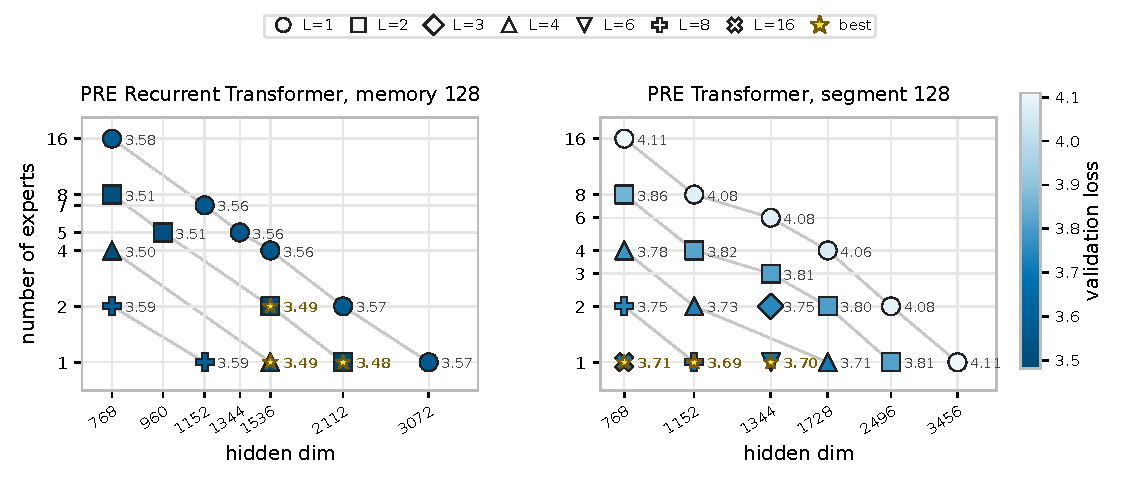
\includegraphics[width=0.88\textwidth]{language_model_recmoe_vs_gptmoe_budget16_128.pdf}
\end{center}
\captionof{figure}{
FineWeb budget-16 comparison at context length 128.
\textbf{Left}: the PRE Recurrent Transformer small-budget allocation map, repeated here for direct comparison. The segment length is 64 and the memory length is 128.
\textbf{Right}: a non-recurrent GPT-style PRE Transformer sweep with training segment length 128 and the same nominal budget.
Color and point labels show validation loss at the latest common logged validation point within each panel, where lower is better; marker shape denotes within-step depth \(L\), and stars mark the best configurations within each panel.
}
\clearpage

\begin{center}
  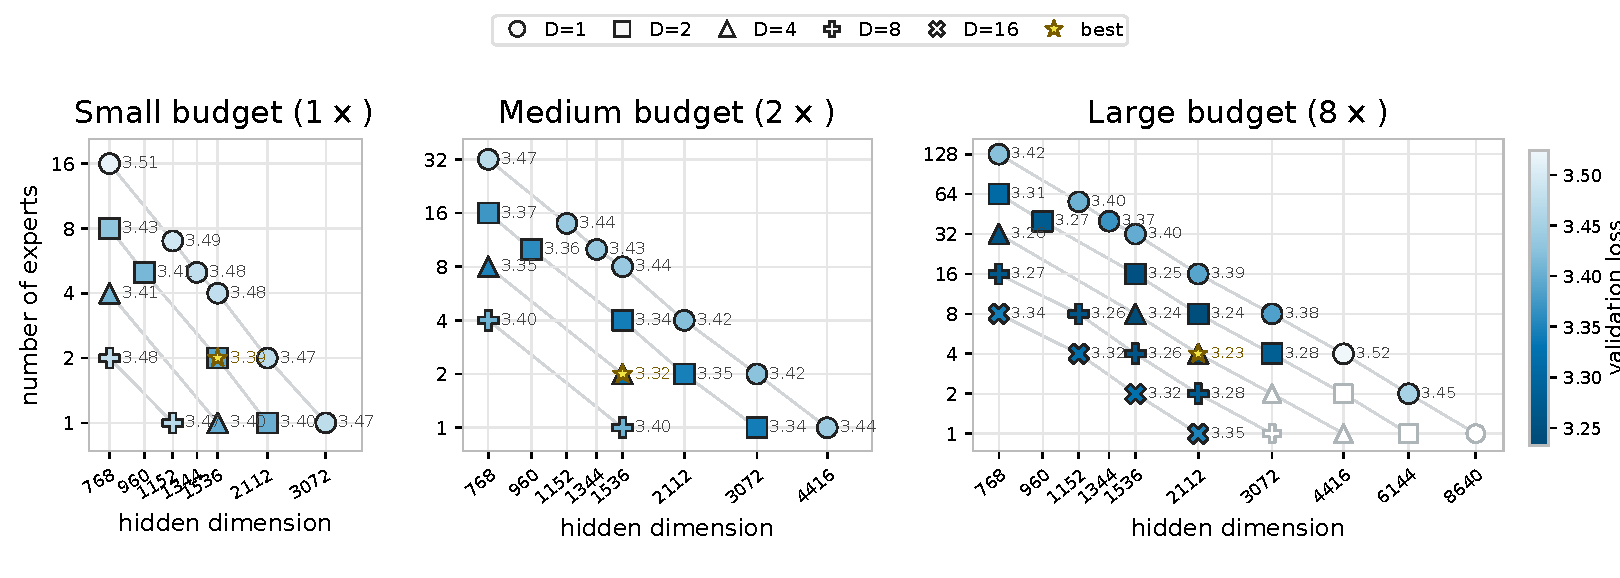
\includegraphics[width=0.90\textwidth]{fineweb_small_medium_large_budget_sandwich_depthshared.pdf}
\end{center}
\captionof*{figure}{
\textbf{Async-paper Figure 2. FineWeb fixed-recurrent-compute allocation across three budgets.}
\textbf{Left:} small budget, with all 14 configurations complete.
\textbf{Middle:} medium budget, twice the small-sweep recurrent compute, with all 16 configurations complete.
\textbf{Right:} large budget, eight times the small-sweep recurrent compute, with 24 of 30 configurations complete, including completed low-expert and depth-16 extensions.
All panels share one validation-loss color scale. Colored points and labels report the final validation checkpoint near 1.295B consumed tokens; all but one use W\&B step 4{,}940, while the lower-PDB \(D=1,E=2,W=6144\) run uses its nearest checkpoint at step 4{,}953. Hollow points mark planned configurations that had not completed when this snapshot was generated.
Circles, squares, triangles, filled-plus markers, and crosses denote \(D=1,2,4,8,16\), respectively; a star marks the best completed configuration in each panel. Lower loss is better. All runs use sequence length 128, memory length 128, a 262{,}144-token optimizer batch, sandwich RMSNorm, and a persistent K/V cache shared across depth. The large panel remains interim while its hollow configurations finish.
}
\vspace{0.7em}

\setcounter{table}{9}
\captionof{table}{
Four-H100 median steady-state decode latency in milliseconds.
GPT-16 uses cached autoregressive decoding with a full sliding-window key-value cache; PRE uses segment-local recurrent decoding with depth-shared recurrent key-value memory. \(B\) is the global batch and \(B/4\) is the per-GPU batch.
}
\begin{center}
\scriptsize
\begin{tabular}{lcc}
  \toprule
  Model & \(C=128,B=16\) & \(C=2048,B=16\) \\
  \midrule
  GPT-16 & 0.636 & 0.760 \\
  PRE \(D=1,E=16\) & 0.133 & 0.209 \\
  PRE \(D=2,E=8\) & 0.498 & 0.645 \\
  PRE \(D=4,E=4\) & 0.694 & 0.943 \\
  PRE \(D=8,E=2\) & 0.943 & 1.447 \\
  PRE \(D=16,E=1\) & 1.465 & 2.454 \\
  \bottomrule
\end{tabular}
\end{center}
\clearpage

\setcounter{table}{10}
\captionof{table}{
Four-H100 FineWeb training throughput in tokens/s.
Each panel fixes token batch \(C B\) and reports segment length \(C\) and global sequence batch \(B\). Values are medians over steps 2--5; startup, compilation, and autotuning steps 0--1 are excluded. OOM denotes measured memory exhaustion. All displayed values use one microbatch per optimizer update.
}
\begin{center}
\scriptsize
\setlength{\tabcolsep}{3.2pt}
\begin{tabular}{lcccccc}
  \toprule
  \multicolumn{7}{c}{131k effective tokens per optimizer update} \\
  \cmidrule(lr){1-7}
  Model & \shortstack{\(C=32\)\\\(B=4{,}096\)} & \shortstack{\(C=64\)\\\(B=2{,}048\)} & \shortstack{\(C=128\)\\\(B=1{,}024\)} & \shortstack{\(C=256\)\\\(B=512\)} & \shortstack{\(C=1024\)\\\(B=128\)} & \shortstack{\(C=2048\)\\\(B=64\)} \\
  \midrule
  GPT-16 & 1{,}004.7k & 1{,}056.6k & 1{,}098.2k & 1{,}113.8k & 1{,}066.1k & 1{,}021.9k \\
  PRE \(D=1,E=16\) & 471.3k & 417.4k & 327.2k & 218.7k & 67.0k & OOM \\
  PRE \(D=2,E=8\) & 229.8k & 182.0k & 128.1k & 79.2k & 22.0k & OOM \\
  PRE \(D=4,E=4\) & 169.0k & 134.6k & 96.7k & 60.6k & 17.1k & OOM \\
  PRE \(D=8,E=2\) & 113.8k & 88.5k & 63.2k & 39.4k & 11.7k & OOM \\
  PRE \(D=16,E=1\) & 68.7k & 54.1k & 37.7k & 24.3k & 7.5k & OOM \\
  \bottomrule
\end{tabular}

\vspace{0.7em}

\begin{tabular}{lcccccc}
  \toprule
  \multicolumn{7}{c}{262k effective tokens per optimizer update} \\
  \cmidrule(lr){1-7}
  Model & \shortstack{\(C=32\)\\\(B=8{,}192\)} & \shortstack{\(C=64\)\\\(B=4{,}096\)} & \shortstack{\(C=128\)\\\(B=2{,}048\)} & \shortstack{\(C=256\)\\\(B=1{,}024\)} & \shortstack{\(C=1024\)\\\(B=256\)} & \shortstack{\(C=2048\)\\\(B=128\)} \\
  \midrule
  GPT-16 & 1{,}115.5k & 1{,}205.6k & 1{,}238.8k & 1{,}245.7k & 1{,}168.6k & 1{,}125.4k \\
  PRE \(D=1,E=16\) & 511.1k & 486.0k & 419.3k & 319.4k & OOM & OOM \\
  PRE \(D=2,E=8\) & 263.7k & 228.7k & 179.4k & 121.7k & OOM & OOM \\
  PRE \(D=4,E=4\) & 193.9k & 166.6k & 131.0k & 90.0k & OOM & OOM \\
  PRE \(D=8,E=2\) & 128.9k & 110.2k & 84.8k & 57.9k & OOM & OOM \\
  PRE \(D=16,E=1\) & 77.9k & 66.3k & 50.5k & 34.1k & OOM & OOM \\
  \bottomrule
\end{tabular}

\vspace{0.7em}

\begin{tabular}{lcccccc}
  \toprule
  \multicolumn{7}{c}{524k effective tokens per optimizer update} \\
  \cmidrule(lr){1-7}
  Model & \shortstack{\(C=32\)\\\(B=16{,}384\)} & \shortstack{\(C=64\)\\\(B=8{,}192\)} & \shortstack{\(C=128\)\\\(B=4{,}096\)} & \shortstack{\(C=256\)\\\(B=2{,}048\)} & \shortstack{\(C=1024\)\\\(B=512\)} & \shortstack{\(C=2048\)\\\(B=256\)} \\
  \midrule
  PRE \(D=1,E=16\) & 543.6k & 517.3k & 477.9k & 377.4k & OOM & OOM \\
  PRE \(D=2,E=8\) & 285.2k & 260.2k & 219.6k & 157.1k & OOM & OOM \\
  PRE \(D=4,E=4\) & 208.2k & 188.9k & 158.9k & 112.0k & OOM & OOM \\
  PRE \(D=8,E=2\) & 137.6k & 124.0k & 103.8k & OOM & OOM & OOM \\
  PRE \(D=16,E=1\) & 83.7k & 74.4k & 60.4k & OOM & OOM & OOM \\
  \bottomrule
\end{tabular}
\end{center}

\end{document}
